% The format (A5) is selected to facilitate reading on small
% devices and should NOT be changed. 
\documentclass[a5paper,10pt,oneside]{article}

% The package babel is loaded for Swdish with Swedish hyphenation,
% replaces "Contents" with "Innehållsförteckning, "References"
% with "Litteraturförteckning", etc.
\usepackage[swedish]{babel}

\usepackage[T1]{fontenc}

% The package "inputenc" lets us specify what character encoding
% has been used to save the .tex file. If your computer runs
% Linux, the encoding is probably "utf8" by default, while under
% Windows the default will probably be "latin1" The wrong
% character encoding may give strange signs instead of "å", "ä"
% and "ö" or may result in compilation errors.

%\usepackage[latin1]{inputenc} % Probably right if you use Windows
\usepackage[utf8]{inputenc}  % Probably right if you use Linux

% The packages listed below are optional and can be removed if you
% don't use them 
\usepackage{graphicx} 
\usepackage{cite}
\usepackage{url}
\usepackage{ifthen}
\usepackage{listings}	


% These two lines set up options for the listings package and
% can be removed if you don't use it, or changed if you, e.g, 
% use another language than Java. 
% For more information about the listings package see:
% ftp://ftp.tex.ac.uk/tex-archive/macros/latex/contrib/listings/listings.pdf
\def \lstlistingname {Kodexempel}
\lstset{language=Java,tabsize=3,numbers=left,frame=L,floatplacement=hbtp}


\usepackage{ifpdf}
\ifpdf
	\usepackage[hidelinks]{hyperref}
\else
	\usepackage{url}
\fi


% Change NR and TITLE below to appropriate values
\title{Tema NR: 4 Hashtabeller}

% Write the name and user namn for all participants in the group here.
% Separate persons with \and
\author{Oscar Törnquist \url{osta3589} \and Emil Rosell \url{emro9957}}



\begin{document}
\maketitle

\section*{Hashfunktion}
En hashfunktion används för att skapa ett värde från indata, som då tilldelas en plats beroende på värdet som blir. Hashfunktionen skapar alltså ett slumpmässigt index inom intervallet. Varje funktion använder sig av en speciell beräkning som görs på den indata som har skickats in, och eftersom dessa algoritmer skiljer sig så måste man veta vilken man ska välja beroende på vad man har för indata. Målet är att ha en funktion som ger varje nyckelvärde en egen plats, vilket kan vara svårt eftersom det finns oändligt många värden en nyckel kan ha, samt platser de kan fördelas på. Man vill dock hitta en funktion som kan göra det så bra som möjligt och som jämt fördelar nyckelvärdena. Vi har konstaterat att inputnycklarna kan vara av olika värden, och därför måste man vara försiktig när man designar en hashfunktion, samt ta hänsyn till olika situationer. Säg att våran indata är integers, då är det vanligt att man gör beräkningen nyckeln mod tabellens storlek. Men det kan innebära problem om nyckelvärdet är besynnerligt. En bra ide som underlättar ifall nyckelvärdet är icke önskvärt är att se till att tabellens storlek är ett primtal. En annan viktig sak att tänka på är att om tabellens storlek är stor så kan det vara svårt att fördela nycklarna på ett bra sätt. Det finns också en risk att nyckelvärdet är väldigt stort, vilket kan medföra att hashfunktionen blir långsam. Ett sätt att lösa detta är att helt enkelt inte använda alla karaktärerna. Genom att bara använda sig av några få karaktärer så sparar hashfunktionen tid.

\section*{Kollisionshanteringsstrategier}
Det finns alltså en risk att två olika nycklar hamnar på samma plats, om ett element som skickas in tilldelas ett värde där det redan finns ett element, detta kallas för kollision. En kollision måste hanteras och det finns olika metoder som hanterar just kollision. De olika kollisionshanteringsstrategierna som finns har olika egenskaper med för och nackdelar, de två vanligaste som används är separate chaining och open addressing.

Vid separate chaining samlas de element som kolliderats i en enkellänkad lista. Platsen där kollisionen har skett blir en pointer till listan. När ett nytt element med samma index kommer hamnar det först i listan. Säg att vi har en tabell med storleken 4 och vi sätter in bokstäverna E, M, I, L. Till exempel får E index 0, M får index 1, I får också index 1,  och L får index 3. På index 1 sker då en kollision som måste hanteras. Index 1 blir en pekare till listan där första elementet är I eftersom I kom efter M. I pekar till det nästa elementet som är M. Om det skulle hamna ett till element på index 1 så läggs det till först i listan.

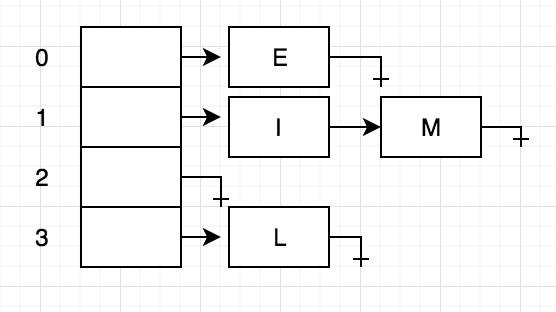
\includegraphics[scale=1]{separate}

Separate chainging är en enkel kollisionshanterare då den använder sig av en länkad lista. Sökning görs genom att gå igenom listan och man kan lägga till fler element än storleken på arrayen. Separate chainging används oftast när man inte vet hur många, och hur ofta ett element läggas till eller tas bort. Användningen av en länkad lista kan dock vara en nackdel eftersom det gör att det går långsammare då den måste allokera nya platser. Vissa platser i hashtabellen kommer heller inte användas vilket är onödigt. Det kan även hända att kedjan blir jättelång vilket leder till att sökningen blir långsam.

Open addressing använder sig av ”probing” för att hantera kollisioner och de vanligaste sätten är Linear probing, Quadratic probing, och Double hashing. Istället för att skapa en länkad lista där elementen sätts in så fortsätter elementet till nästa plats till dess att den kommer till en plats som är tom. Detta gör att storleken på arrayen måste vara betydligt större än om man använder sig av separate chainging.

 I Linear probing går man ett steg i taget till nästa index och detta görs till dess att en tom plats hittas och elementet hamnar då där. Om vi säger att hash(x) är indexet där kollistionen sker, så gör linear probing hash(x) + 1 för att gå till nästa plats, är den platsen upptagen så gör den hash(x) + 2 osv tills den hittar en tom plats . Problemet med linear probing är att det kan blidas clustering, då fler element hamnar tillsammans i väntan på element som söker efter en tom plats. 
 
 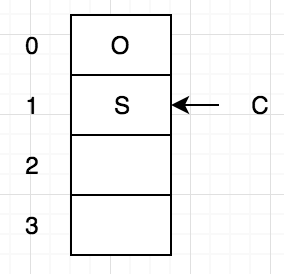
\includegraphics[scale=1]{prob1}
 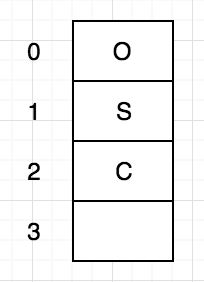
\includegraphics[scale=1]{prob2}
 
 På bilden sätter vi förs in ett O på index 0 och ett C på index 1. När vi sedan sätter in C så sker en kollision på index 1. Vid användning av linear probing går C vidare till nästa index som visar sig vara tom och hamnar då där.

Quadratic probing använder sig istället av funktionen $f(i) = i^2$  för att hitta en tom plats. Detta minskar risken för clustering. Om det sker en kollision så beter sig quadratic probing genom att ta hash(x) + 1*1, sedan hash(x) + 2*2, osv tills dess att den har hittat en tom plats åt elementet. 

 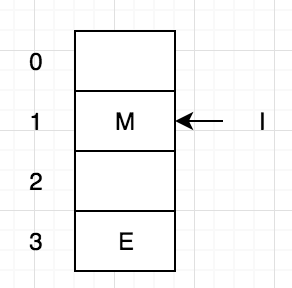
\includegraphics[scale=1]{Qua2}
 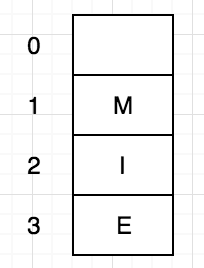
\includegraphics[scale=1]{Qua1}
 
 På bilden har vi satt in ett E på index 3 och M på index 1. När vi sedan sätter in I får vi en kollision på index 1. Vi använder oss då av quadratic probing(hash(x) + 1*1) och hamnar på index 2. Skulle platsen vara upptagen skulle vi fortsätta och ta $2^2$ vilket blir 4, och kolla om platsen som är fyra platser bort är tom, annars ta $3^3$ vilket blir 6, och kolla om platsen som är sex platser bort är tom, osv tills vi hitter en tom plats.
 
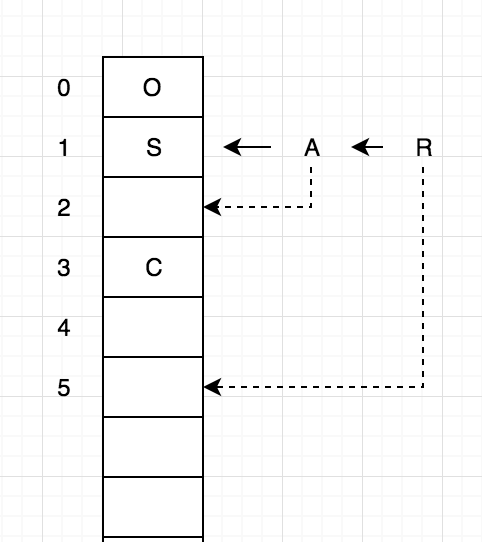
\includegraphics[scale=1]{quad}

I ett till exempel lägger vi först till O, S, C, sedan när vi lägger till A så sker en kollision på index 1. Med användning av quadratic probing hamnar A på index 2, eftersom index 1 + 1*1 blir 2. När vi sedan lägger till R så sker en kollision på index 1 igen. Då använder vi quadratic probing igen och först görs index 1 + 1*1, men där har vi redan A, så vi går vidare och det sker index 1 + 2*2, vilket blir 5. index 5 är tom så R hamnar där.

Double hashing använder sig istället av en till hashfunktion för att hitta en tom plats. Den använder sig då av funktione $f(i) =  i*hash2(x)$. Det första som händer då är att den tar hash(x) + 1*hash2(x) och sedan hash(x) + 2*hash2(x), osv tills den hittar en tom plats. Den använder sig alltså av den andra funktionen för att hitta en tom plats. Vid linear och quadratic probing kommer värden som kolliderar alltid leta efter en tom plats på samma ställen. Som i bilden ovan letar både A och R på index 2 först, och sedan index 5 osv tills en tom plats har hittat. Vid Double hashing kommer letandet efter en tom plats bero på värdet hos nyckeln som kollideras. A kan kan hamna på nått helt annat index, likaså R. Endast nycklar av samma värde kommer leta på samma platser. Vid Double hashing sker då ingen clustering men det krävs mer minne eftersom det används två funktioner.

\end{document}
